\subsection{Mass distribution from Lensing}

\paragraph{Best fit lens model.} The best fit lens model for the image positions in tab. \ref{tab:lenspos} is given in the first column of tab. \ref{tab:bestfitlensmodel}. Fig. \ref{fig:lensbestfiteinsteincurves} shows the corresponding critical curve, caustic and Einstein radius, and the best fit source position. In this case, where $\alpha=1$, the critical curve is also an equidensity contour of the galaxy model. Fig. \ref{fig:lensbestfittimedelay} overplots the smoothed residuals from the F814W image subtracted by the IRAF ellipse fit to the surface brightness with the contours of the best fit model's time delay surface. This demonstrates that, although we did not include any information about the shape of the lensing images in the fit, it is consistent with the predicted distortion for an extended source by the best fit lens model.
\\To estimate how the uncertainties in the determination of the image positions and galaxy center affect the results, we Monte Carlo sample random positions from a two-dimensional Normal distribution centered at the positions in tab. \ref{tab:lenspos} and a standard deviation corresponding to the measurement error of 1 pixel. A Gaussian fit to the resulting distributions of best fit values leads to the constraints on the shape parameters and Einstein quantities in the second column in tab. \ref{tab:bestfitlensmodel}. We therefore constrain the Einstein radius to within 2\%, $R_\text{ein} = (0.91 \pm 0.02)$ arcsec and the projected mass within the critical curve with a relative error of 4\%, $M_\text{crit} =(7.9\pm0.3)\cdot 10^{10} M_\odot$. Our measurement of $R_\text{ein}$ is consistent with that from \citet{SWELLSIII}, $R_\text{ein,SWELLS} = (0.96 \pm 0.04)$ arcsec. The relative difference between our critical mass and that of \citet{SWELLSIII}, $M_\text{crit,SWELLS} =(8.86\pm0.61)\cdot 10^{10} M_\odot$, is 13\%.

%========================================================================================

\begin{table*}
\centering
\caption{??? in tab. \ref{tab:lenspos}, for $\alpha = 1$}
\begin{tabular}{llrrclr}
\hline
 &  & \multicolumn{1}{c}{lens model for} &\multicolumn{4}{c}{lens model from Monte Carlo sampling  } \\
 &  & \multicolumn{1}{c}{peak image positions}  & \multicolumn{4}{c}{of image positions }  \\ \hline
Einstein Radius      & $R_\text{ein}$ [arcsec]             & $0.907$ & $0.91$  & $\pm$ & $     0.02$ & ($2\%$)\\
Einstein Mass        & $M_\text{ein}$ [$10^{10} M_\odot$]  & $7.72$  & $7.8 $  & $\pm$ & $      0.3$ & ($4\%$) \\
Critical Mass        & $M_\text{crit}$ [$10^{10} M_\odot$] & $7.87$  & $7.9$   & $\pm$ & $      0.3$ & ($4\%$)\\
Source Position      & $\xi$ [arcsec]                      & $0.095$ & $0.09 $ & $\pm$ & $     0.03$ & ($28\%$)\\
                     & $\eta$ [arcsec]                     & $0.107$ & $0.10 $ & $\pm$ & $     0.03$ & ($27\%$)\\
Fourier Coefficients & $a_0$                               & $1.814$ & $1.82 $ & $\pm$ & $   0.04$ & (2\%)\\
                     & $a_2$                               & $0.012$ & $ 0.011 $ & $\pm$ & $    0.004$ & (35\%)\\
                     & $b_2$                               & $-0.057$ & $-0.06 $  & $\pm$ & $  0.01$ & (25\%)\\
                     & $a_3$                               & $-0.0001$& $0.0000 $ & $\pm$ & $   0.0006$ & \\
                     & $b_3$                               & $-0.0002$&$0.000 $   & $\pm$ & $  0.001$ & \\\hline
\end{tabular}  
\label{tab:bestfitlensmodel} 
\end{table*}

%========================================================================================

\begin{figure*}
\centering
\begin{subfigure}{.5\textwidth}
  \centering
  \includegraphics[width=.9\linewidth]{fig/lens_einstein.ps}
  \caption{??? Critical curves, Einstein radius, caustics, source position for best fit model. ??? [TO DO: nice caption]}
  \label{fig:lensbestfiteinsteincurves}
\end{subfigure}%
\begin{subfigure}{.5\textwidth}
  \centering
  \includegraphics[width=.9\linewidth]{fig/lens_timedelay.ps}
  \caption{??? Time delay surface ??? [TO DO: nice caption]}
  \label{fig:lensbestfittimedelay}
\end{subfigure}
\caption{???}
\label{fig:???}
\end{figure*}

%========================================================================================

\paragraph{Comparison with Light Distribution.} Fig. \ref{fig:lenscomparemass} shows the surface mass distribution as predicted by the best fit model in tab. \ref{tab:bestfitlensmodel}. We introduce random noise according to the uncertainties in the Fourier shape parameters to create a mock observation that visualizes the effect of the measurement errors. To be able to compare the predicted mass distribution to the observed light distribution we transform the surface brightness into a mass density: We first integrate the MGE in tab. \ref{tab:MGEF814W} to get the total luminosity within the Einstein radius and the predicted mass-to-light ratio as $\Upsilon_\text{I,ein} = M_\text{ein} / L_\text{I,ein}$. Fig. \ref{fig:lenscomparelight} shows then the observed surface brightness in the F814W filter multiplied by $\Upsilon_\text{I,ein}$.  Fig. \ref{fig:lenscompareboth} finally compares equidensity contours at the same values of both the predicted lens mass distribution and the observed surface brightness times $\Upsilon_\text{I,ein}$. We note the following three facts: 1.The mass predicted from lensing and the observed light distribution are oriented in the same direction. 2. Within the Einstein radius mass and light distribution have the same shape, while further out the mass distribution is more roundish. 3. The light distribution drops faster than the mass with increasing radius. This could indicate that the stellar component of the galaxy is superimposed by a more roundish dark matter component.

\paragraph{[TO DO: Stuff to mention]}
\begin{itemize}
\item best fit lens total mass distribution of J1331 has the same position angle and a similar elliptical shape as the surfache brightness distributon, but is slightly rounder, and could be consistent with a flat rotation curve.
\end{itemize}

%========================================================================================

\begin{table}
\centering
\caption{???}
\begin{tabular}{cc}
\hline
Total I-band luminosity within $R_\text{ein}$ & Mass-to-light ratio within $R_\text{ein}$\\
 $L_\text{I,ein}$ [$10^{10} L_\odot$] & $\Upsilon_\text{I,ein} = M_\text{ein} / L_\text{I,ein}$ [$\Upsilon_\odot$]\\\hline
1.40 & 5.56\\\hline
\end{tabular}  
\label{tab:einsteinML} 
\end{table}

%========================================================================================

\begin{figure*}
\centering
\begin{subfigure}{.3\textwidth}
  \centering
  \includegraphics[width=.9\linewidth]{fig/lens_surface_brightness.ps}
  \caption{???}
  \label{fig:lenscomparelight}
\end{subfigure}%
\begin{subfigure}{.3\textwidth}
  \centering
  \includegraphics[width=.9\linewidth]{fig/lens_surface_density.ps}
  \caption{???}
  \label{fig:lenscomparemass}
\end{subfigure}
\begin{subfigure}{.3\textwidth}
  \centering
  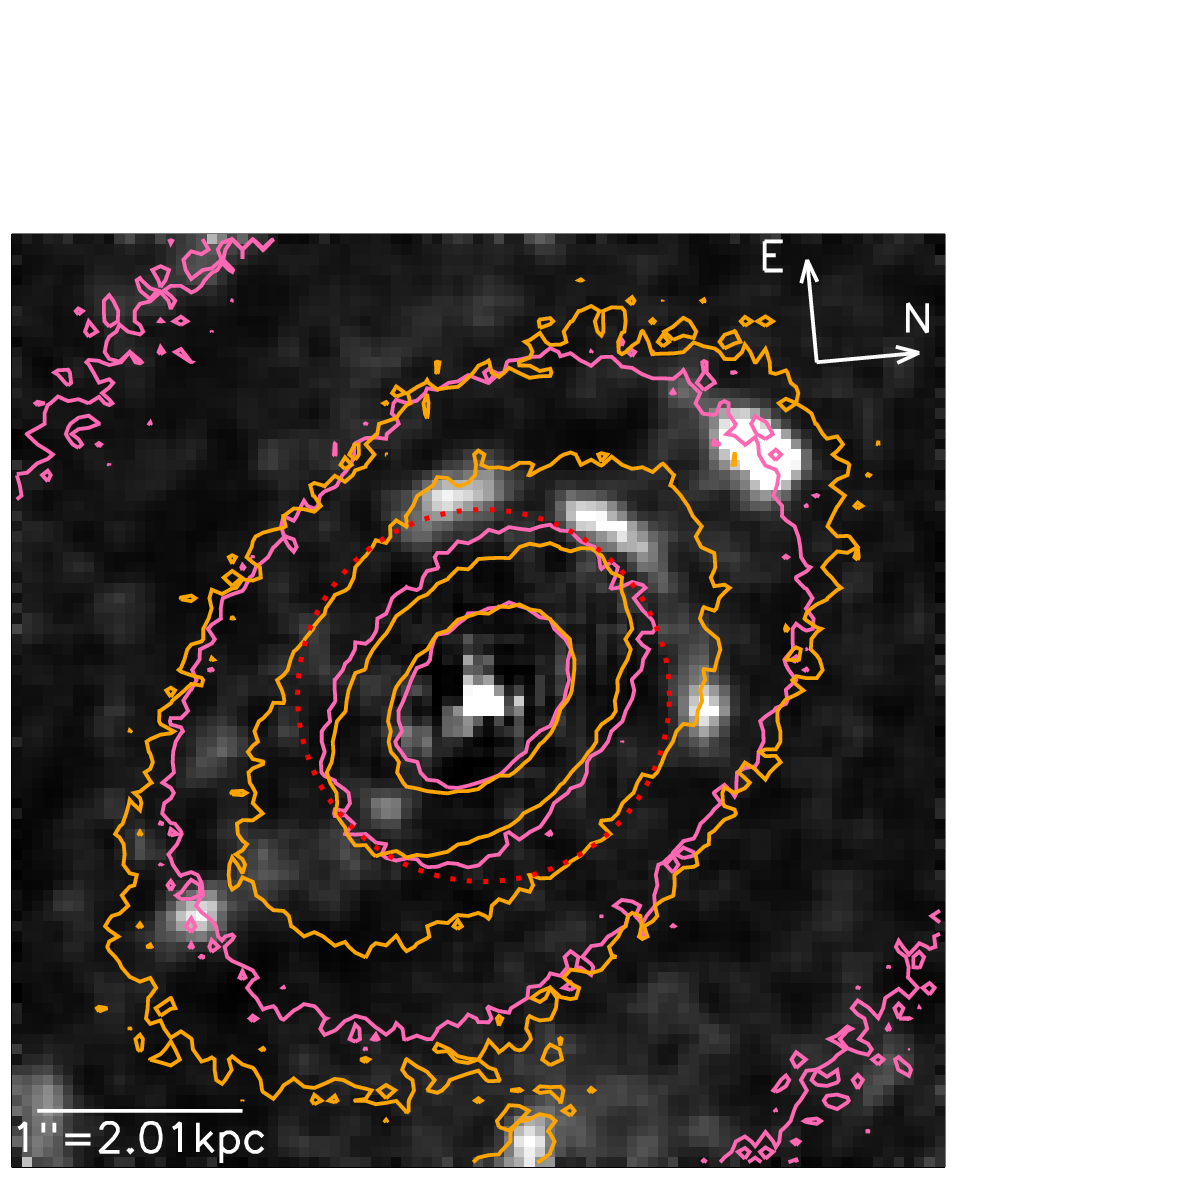
\includegraphics[width=.9\linewidth]{fig/paper_lensmass_brightness_compare.ps}
  \caption{???}
  \label{fig:lenscompareboth}
\end{subfigure}
\caption{??? Preliminary crappy caption: Left: OBSERVED surface bightness multiplied with M/L in Einstein radius (overplotted in red). Middle: BEST FIT MODEL for mass distribution from lensing (including "wriggles" due to uncertainties in image positions). Contours are at the same levels. Right: Same contours, to directly show the difference in shape. ??? [TO DO: nice caption]}
\label{fig:???}
\end{figure*}


